\documentclass[12pt]{article}
\usepackage{amsmath}
\usepackage{url}
\usepackage{graphicx}
\graphicspath{{./img/}}
\usepackage{wrapfig}
\usepackage[numbers]{natbib}
\usepackage[czech]{babel}
\usepackage[T1]{fontenc}
\usepackage[utf8]{inputenc}
\title{FI-HMI: Temperovaná ladění}
\date{\today}
\author{Adam Havel}
\begin{document}

\maketitle

\pagebreak

\section{Absolutní a relativní sluch}

Každý alespoň trochu schopný muzikant by měl disponovat dobrým relativním sluchem, tedy schopností poznat frekvenční rozdíl mezi dvěma znějícími tóny a jen na základě poslechu rozhodnout, jaký hudební interval je odděluje. Takových intervalů je alespoň v naší klasické hudební nauce dvanáct, což je přirozeně stejné množství, jaké nám nabízí repertoár hudebních tónů neboli chromatická řada. A právě umění rozpoznat krom intervalu i samotné absolutní výšky, to znamená přiřadit je k jednomu z těchto dvanácti tónů — jako třeba C nebo G$\flat$ — se nazývá absolutním sluchem.

Většina lidí má představu, že je tato schopnost vrozená a spojuje si ji s jakýmsi přirozeným hudebním nadáním — ostatně jako příklad člověka, který byl tímto sluchem obdařen, se často udává třeba Wolfgang Amadeus Mozart. Jak ovšem zjistíme, s tímto \uv{Svatým grálem} muzikantů to není tak úplně jednoduché.

Dnes už tušíme, že se absolutní sluch formuje především v raném dětství a hlavní faktor představuje opakované vystavení hudebním tónům spolu s dalším podnětem, třeba vizuálním, který ke konkrétním zvukům přiřadí dané označení. Dětský mozek je pak schopen toto spojení zachovat a slyší-li pak jedinec, u kterého se tato vlastnost projeví, správnou frekvenci, na mysl mu okamžitě vytane i název tónu.

Problém ovšem nastane v momentě, kdy si uvědomíme, že frekvence jednotlivých tónů jsou jen předmětem úzu a momentální dohody a jejich hodnoty se tedy v průběhu času významně mění. Dnes se jako reference pro lazení nástrojů většinou používá tzv. koncertní A o hodnotě 440 Hz, nicméně to samé A bylo na počátku předchozího století skoro o deset hertzů menší. Podíváme-li se až do osmnáctého století, zjistíme dokonce, že se tato frekvence významně lišila nejen v čase, ale například i v rámci různých měst, a to i o desítky hertzů \cite{wiki_pitch}!

Ve světle těchto zjištění se absolutní sluch jeví jako svého druhu Danajský dar. V momentě, kdy orchestr ladí jinak, než je dnes zvyklé — třeba z důvodu větší autentičnosti u současných barokních souborů — pak člověk s absolutním sluchem narozdíl od běžného posluchače tento rozdíl slyší a nepříjemně pociťuje. Nicméně, ani běžní lidé nejsou ušetřeni následků změn hudebního úzu, protože se mění nejen tóny, ale i samotné vzdálenosti mezi nimi. Tyto intervaly určuje matematicky odvozený systém nazvaný ladění, kterých v historii vzniklo velké množství: v hudební tradici naší západní kultury například dominuje takzvané rovnoměrně temperované ladění. Tak to ovšem nebylo vždy.

\pagebreak

\section{Harmonická řada}

Hudba, jak ji známe, by nemohla existovat nebýt jedné vlastnosti lidského mozku, a to sice té, že dva tóny vnímá jako v podstatě stejné, pokud jsou od sebe vzdáleny o interval oktávy. To jinými slovy znamená, že jsou jejich frekvence členy stejné geometrické posloupnosti o kvocientu 2 — jako A jsou tedy shodně označeny například tóny o frekvenci 440 a 220 Hz. Tuto vlastnost mimochodem sdílíme s mnoha dalšími savci \cite{octave_circularity}.

Ladění pak není nic jiného, než způsob, jak takto daný frekvenční rozsah rozdělit na jednotlivé tóny. Zde je důležité poznamenat, že ačkoliv v naší kultuře jsme zvyklí (už od Pythagora!) používat tónu dvanáct, jejich množství — ač podstatné — není pevně dané.

\begin{wrapfigure}{l}{0.4 \textwidth}
\centering
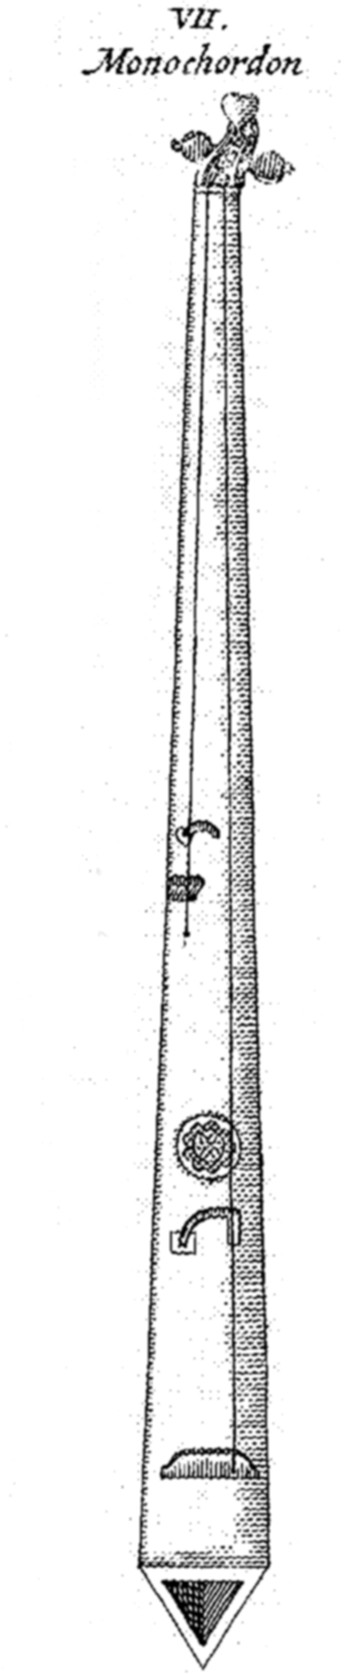
\includegraphics[width = 0.1 \textwidth]{monochord.jpg}
\caption{Monochord}
\label{fig:monochord}
\end{wrapfigure}

Právě Pythagorovi se pak přisuzuje jedno z nejstarších známých ladění, které se hojně používalo až do 16. století \cite{smolka}. Rozložení tónů v tomto systému bylo založeno na pozorování takzvaného \emph{monochordu}, což byl jednoduchý hudební — nebo spíše vědecký — nástroj o jedné (či více) strunách, určený k demonstraci vlastností tónů. S jeho pomocí tedy mohli zkoumat třeba výše zmíněnéný interval oktávy, a to tak, že strunu zkrátili na polovinu, čímž se frekvence tónu zdvojnásobila.

Řekové si tehdy všimli, že struna uchycená na dvou koncích vibruje s frekvencí o vlnové délce rovné dvojnásobku délky struny — této frekvenci se říká \emph{fundemantální}. Ovšem mnohem důležitější bylo zjištění, že struna zároveň vibruje i s dalšími frekvencemi. Další z nich má vlnovou délku rovnou délce struny, její frekvence je tedy dvákrat tak velká, což znamená, že jde o interval oktávy. Vibruje-li tedy struna s frekvencí 100 Hz, vibruje zároveň i s frekvencí 200 Hz. Tímto způsobem dělení struny pokračuje a jako další pozorujeme vibraci o 300 Hz, která je s předchozí oktavou v poměru 3:2 a jedná se o interval čisté kvinty. Jak můžeme vidět na obrázku ~\ref{fig:harmonics}, další frekvence je zase oktáva o frekvenci 400 Hz a až poté následuje nový tón o 500 Hz. Ten je s předchozí oktávou v poměru 5:4, jde tedy o velkou tercii. Následuje další kvinta a tak dále.

Tyto tóny se označují jako \emph{alikvótní} a jejich funkce je naprosto zásadní, protože jejich množství a intenzita v poměru k fundamentálnímu tónu vytvářejí takzvanou barvu tónu. A právě díky barvě jsme jen podle sluchu schopni poznat hudební nástroj jeden od druhého. Některé, třeba flétna, disponují jen alikvótními tóny oktávy, jiné zase jen těmi lichými a podobně.

\begin{figure}[p]
\centering
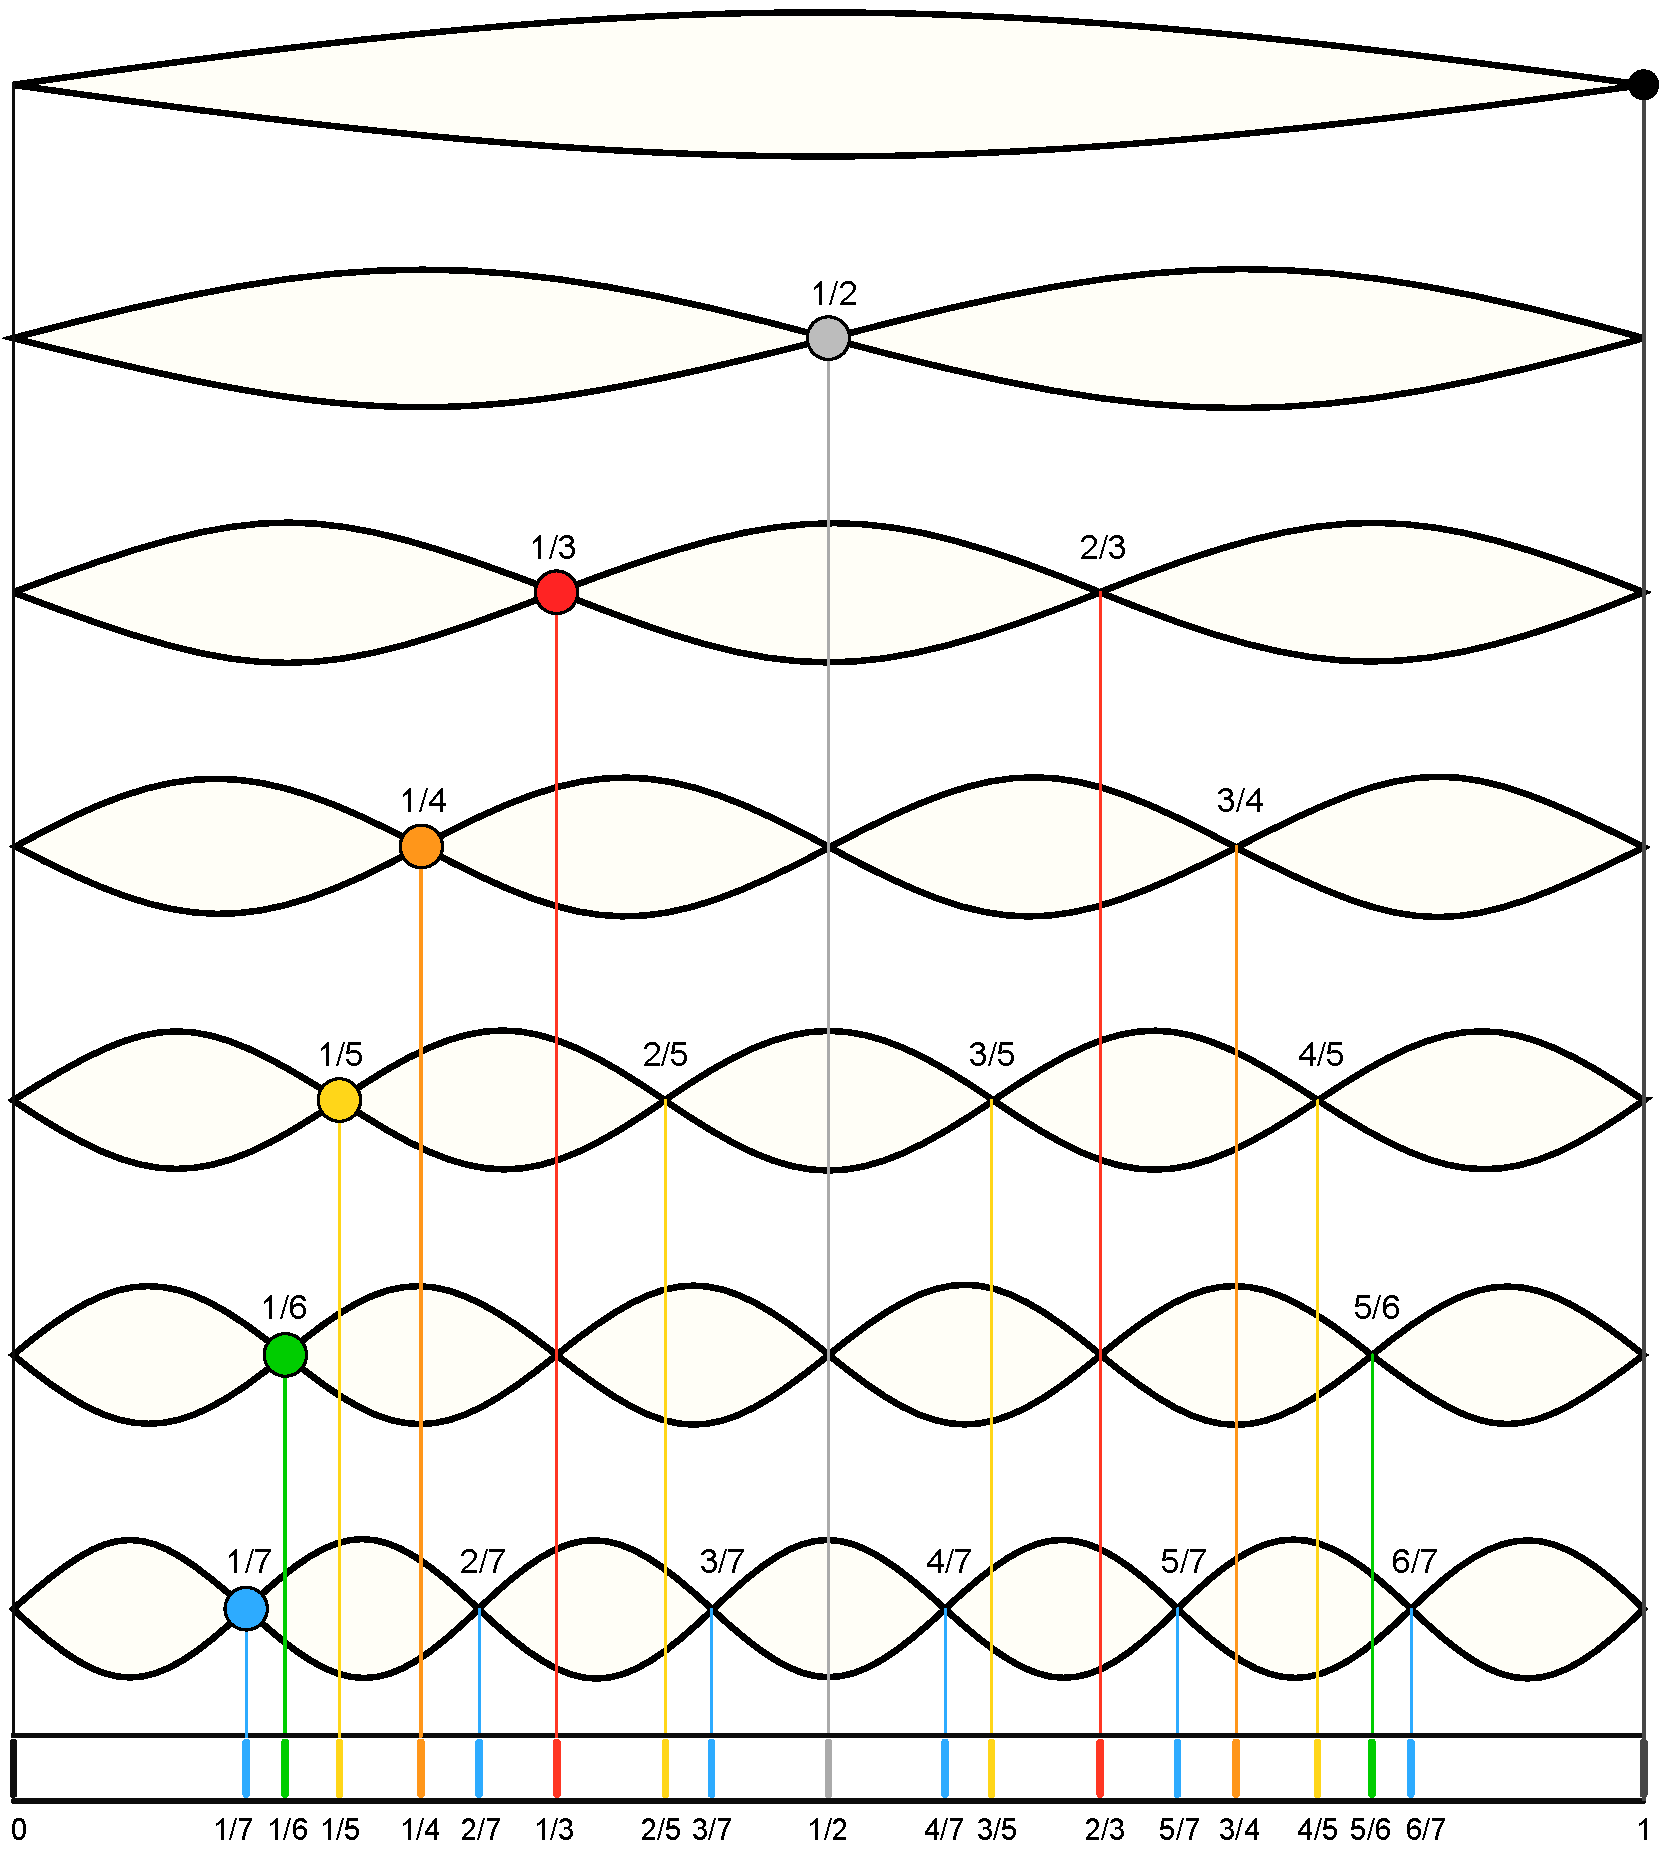
\includegraphics[width = .9 \textwidth]{harmonics.pdf}
\caption{Harmonická řada (zdroj: Wikimedia)}
\label{fig:harmonics}
\end{figure}

Než budeme pokračovat dále, je třeba si uvědomit několik poznatků. Zaprvé, alikvótní tóny jsou zjevně členy aritmetické posloupnosti o diferenci rovné fundamentální frekvenci. Zadruhé, vyšší oktávy a kvinty jsou nedílnou a podstatnou součastí většiny vibrujících těles. A zatřetí, jak postupujeme v harmonické řadě, objevují se stále menší intervaly a zlomky vyjadřující poměr k oktávám jsou čím dál složitější. Čistá kvinta s poměrem 3:2 je pak tedy hned po oktávě nejjednodušší interval. To je důležite i proto, že náš mozek vnímá intervaly, které se dají vyjádřit pomocí poměru malých čísel, jako uklidňující. Naproti tomu ty intervaly, které mají ve zlomku velká čísla, považuje za nepříjemné.

Není proto náhodou, že nejstarší pentatonické stupnice (stupnice o pěti tónech) jsou založeny právě na intervalech přirozeně se vyskytujících v přírodě v podobě alikvótních tónů. Krom oktávy a kvinty jsou to velká tercie, čistá kvarta a malá septima. O tercii jsme se již zmínili, zaměříme se proto na poslední dva. Kvarta se ve skutečnosti v harmonické řadě objevuje až jako dvacátý alikvótní tón, ale dá se jednoduše matematicky odvodit ze svého vztahu ke kvintě. Jde totiž o její inverzi, což znamená, že složíme-li dohromady interval kvinty a kvarty, dostaneme oktávu. Víme-li, že kvinta je v poměru 3:2 a oktáva 2:1, můžeme si lehce odvodit, že kvarta představuje zlomek 4:3.

S přirozenou malou septimou je to složitější. Ta se v harmonické řadě objevuje jako šestý člen o poměru 7:4, což je pomerně odlišné číslo, než k jakému matematicky dospěli Řekové nebo jaké dnes používáme my v temperovaném ladění. Proto by se na dnešním klavíru tento interval zahrát nedal, neboť by ležel někde mezi velkou sextou a malou septimou. Jeho velikost se lišila i v rámci různých kultur, například v čínské tradici se používal interval srovnatelný s naší dnešní malou septimou, zatímco v té africké to naopak byla spíše velká sexta \cite{bernstein}.

\section{Čistá ladění}

S předchozími znalostmi se konečně můžeme vrátit k Pythagorovi a jeho ladění, jehož základy stojí právě na intervalech oktávy a kvinty.  

\pagebreak

Harmonická řada (vibrace, barva nástroje)

Pentatonika (šestý alikvótní tón, oktávy)

Přirozené ladění (Pythagorejské, Didymické, enharmonické intervaly, kvintový kruh)

Baroko a cembalo (modulace, Bach, dur-mollové harmonie, konsonantní tercie a kvintakordy)

Temperovaná ladění (rozdílnost tónin)

Rovnoměrně temperované ladění (důvod, důsledky, matika)

Současnost


\bibliography{sources}{}
\bibliographystyle{plainnat}

\end{document}